

\tikzset{every picture/.style={line width=0.75pt}} %set default line width to 0.75pt        

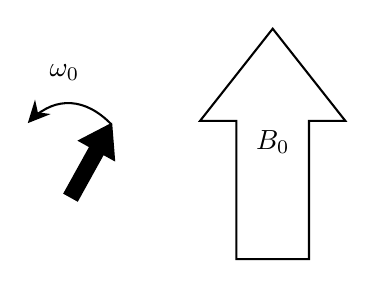
\begin{tikzpicture}[x=0.75pt,y=0.75pt,yscale=-1,xscale=1]
%uncomment if require: \path (0,300); %set diagram left start at 0, and has height of 300

%Up Arrow [id:dp2876681549745119] 
\draw   (134,99.9) -- (169,55.5) -- (204,99.9) -- (186.5,99.9) -- (186.5,166.5) -- (151.5,166.5) -- (151.5,99.9) -- cycle ;

%Up Arrow [id:dp5678377322053672] 
\draw  [fill={rgb, 255:red, 0; green, 0; blue, 0 }  ,fill opacity=1 ] (75.94,109.44) -- (91.2,101.51) -- (92.56,118.65) -- (87.33,115.75) -- (74.89,138.2) -- (68.72,134.78) -- (81.16,112.33) -- cycle ;
%Curve Lines [id:da6969268383286944] 
\draw    (91.2,101.51) .. controls (78.73,88.74) and (64.64,88.04) .. (53.01,98.97) ;
\draw [shift={(51,101)}, rotate = 312.71000000000004] [fill={rgb, 255:red, 0; green, 0; blue, 0 }  ][line width=0.08]  [draw opacity=0] (10.72,-5.15) -- (0,0) -- (10.72,5.15) -- (7.12,0) -- cycle    ;

% Text Node
\draw (159.5,102.9) node [anchor=north west][inner sep=0.75pt]    {$B_{0}$};
% Text Node
\draw (60,71.4) node [anchor=north west][inner sep=0.75pt]    {$\omega _{0}$};


\end{tikzpicture}
